% 2018 浙江卷第19题：多面体立体几何示意图
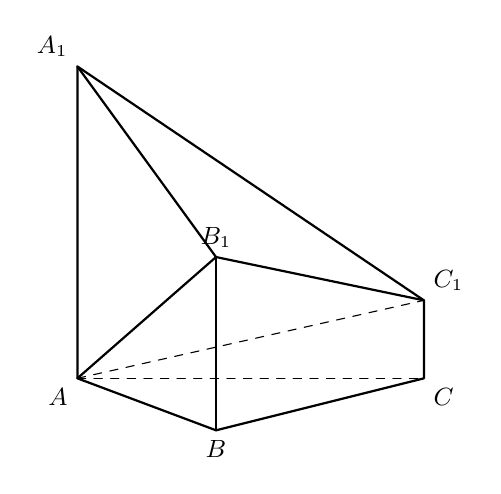
\begin{tikzpicture}[font=\small, line cap=round, line join=round, >=stealth, scale=1.1]
  % 顶点定义
  \coordinate (A) at (0, 0);
  \coordinate (B) at (1.6, -0.6);
  \coordinate (C) at (4.0, 0);
  \coordinate (A1) at (0, 3.6);
  \coordinate (B1) at (1.6, 1.4);
  \coordinate (C1) at (4.0, 0.9);

  % 虚线（隐藏棱）
  \draw[dashed, thin] (A) -- (C);
  \draw[dashed, thin] (A) -- (C1);

  % 实线（可见棱）
  \draw[thick] (A1) -- (A) -- (B) -- (C) -- (C1) -- cycle;
  \draw[thick] (B) -- (B1);
  \draw[thick] (A1) -- (B1) -- (C1);
  \draw[thick] (A) -- (B1);

  % 顶点标签
  \node[above left] at (A1) {$A_1$};
  \node[above] at (B1) {$B_1$};
  \node[above right] at (C1) {$C_1$};
  \node[below left] at (A) {$A$};
  \node[below] at (B) {$B$};
  \node[below right] at (C) {$C$};
\end{tikzpicture}
